\documentclass[article,11pt,oneside,a4paper]{abntex2} % a4paper, twocolumn se quiser duas colunas

\usepackage[utf8]{inputenc} %para funcionar acentuação em portugues
\usepackage{graphicx} %pacote para inserir imagens
\usepackage{mathtools} %pacote para inserir equações
%\usepackage[square,sort,comma]{natbib} %pacote para gerenciar referências bibliográficas.
\usepackage[alf,bibjustif]{abntex2cite}
\usepackage{adjustbox}
\usepackage{listings}
\renewcommand{\lstlistingname}{Código}% Listing -> Algorithm
\renewcommand{\lstlistlistingname}{List of \lstlistingname s}% List of Listings -> List of Algorithms



 
\date{}

\begin{document}
	\pagestyle{plain}
	
	\title{\Large Visualização de dados pluviométricos com utilização de Banco de Dados não relacional.}
	\author{\large Guilherme H. L. dos Santos \hspace{.25cm} \large Milton H. Shimabukuro\\
		Departamento de Matemática e Computação - Universidade Estadual Paulista (UNESP)\\
		19.060-900 - Presidente Prudente - SP - Brasil\\
		g.lourenco.santos@gmail.com, miltonhs@fct.unesp.br}

	\maketitle
	
	\renewcommand{\abstractname}{Abstract} 
	\begin{abstract}

	In this work, visualization techniques were applied to pluviometric data obtained from measurement stations, it was added interactivity and ways to show the visualizations simultaneously and coordinated, so that more information could be obtained. As support, the javascript library D3.js was used for data-oriented visualization, and the management of the data was done by PostgreSQL, with the JSONB document-oriented NoSQL feature, seeking to better adapt to the data type, using a hybrid approach joining to a relational database with non-relational resources. A WEB environment was built and, through the visualizations, it was possible to extract information about rain averages at various time scales, the consistency periods of the rainfall data of each station, the monthly rainfall behavior of several stations, and the space positioning of the stations. And it was possible to associate this informations through the simultaneous and coordinated presentation of the visualizations. It was also possible to analyze the use of the hybrid approach to data management, and the use of the D3.js library to construct the visualizations.

	\end{abstract}

	\renewcommand{\abstractname}{Resumo} 
	\begin{abstract}
		Neste trabalho, técnicas de visualização foram aplicadas a dados pluviométricos obtidos de diversas estações de medição, utilizando interatividade, e disponibilizando visualizações simultâneas e coordenadas, para que mais informações pudessem ser obtidas. Como apoio, foi utilizada a biblioteca javascript D3.js, para visualização orientada a dados, e a gerência dos mesmos foi feita pelo PostgreSQL, com o recurso NoSQL orientado a documento JSONB, buscando melhor se adaptar ao tipo dos dados, utilizando uma abordagem híbrida unindo uma base de dados relacional com recursos não relacionais. Então foi construído um ambiente WEB em que, através das visualizações, foi possível extrair informações sobre as médias de chuva em diversas escalas temporais, o períodos de consistências dos dados pluviométricos de cada estação, o comportamento mensal de chuvas de diversas estações, e o posicionamento espacial das estações, sendo possível associar estas informações através da apresentação simultânea e coordenada das visualizações. Foi possível também analisar o uso da abordagem híbrida para a gerência dos dados, e o uso da biblioteca D3.js para construir as visualizações.
		
	\end{abstract}

	\section{Introdução}
	\hspace{13pt}
	A análise de dados pluviométricos é de grande importância pois é uma variável dentro de diversos estudos sobre fenômenos da natureza, estando conectada a diversos fatores como a erosão de solos, o enchimento de rios, o comportamento da fauna e flora, e dentre outros, com aplicações em diversas áreas como nos setores agrícolas e agropecuários, de transporte aéreo, rodoviário e naval, de saneamento, e outros \cite{crepani2004intensidade}, \cite{oliveira2009importancia}, \cite{assad1998sistema}. Os dados de chuva são capturados por várias estações de medição na escala diária, e podem ser analisados dia a dia, mês a mês, ano a ano e, eventualmente, analisa-se os dados em todas as escalas ao mesmo tempo. Tais dados também podem ser muito volumosos, e de complexa recuperação dentro de algumas bases de dados.
	
	Devido ao volume de dados e diferentes formas de análise em diferentes escalas de tempo, é importante que exista uma maneira de visualizar vários dados pluviométricos ao mesmo tempo de forma clara e estruturada, conforme alguns trabalhos, tais como o de \citeonline{branco2003visualizacao} que utilizou a visualização para explorar dados pluviométricos, de  \citeonline{romero2015herramienta} que utilizou a visualização para correntes de vento em um ambiente WEB com o uso do D3.js\footnote{https://d3js.org/, acessado em 7 de Agosto de 2017} e de \citeonline{genghini} que incorporou recursos de interatividade a uma plataforma de visualização já existente, é possível observar que a visualização por meio de ferramentas computacionais pode auxiliar nestas análises, como o uso do  JavaScript\footnote{http://www.ecma-international.org/publications/files/ECMA-ST/Ecma-262.pdf, acessado em 7 de Agosto de 2017}(linguagem de programação baseada em \textit{scripts}) com a biblioteca D3.js para gerar imagens SVG(\textit{Scalable Vector Graphics}). O volume dos dados também pode influênciar na maneira de armazená-los e recuperá-los para a apresentação e interação, então é importante que haja uma forma adequada para fazê-lo. O uso de banco de dados não relacionais pode ser uma opção que viabilize este processo, pois tem obtido sucesso em diversas aplicações com grande volume de dados como: Facebook\footnote{https://www.facebook.com/, acessado em 15 de Agosto de 2017}, Google\footnote{https://www.google.com.br/, acessado em 15 de Agosto de 2017} e Twitter\footnote{https://twitter.com/, acessado em 15 de Agosto de 2017}.
	
	Existe também um número grande e crescente de diferentes plataformas de software e de diferentes dispositivos computacionais em uso \cite{cisco}, o que torna o desenvolvimento de aplicações presentes em todos mais difícil, e com um alto consumo de tempo neste desenvolvimento devido a diferença de sistemas operacionais com diferentes linguagens de programação especificas para cada um \cite{chmielewski2014device}. Uma possível solução para este problema seria a construção de aplicações WEB\footnote{https://www.w3.org/2008/webapps/, acessado em 7 de Agosto de 2017}, pois se baseiam em aplicações que utilizam os navegadores\footnote{https://www.w3.org/TR/webarch/, acessado em 7 de Agosto de 2017} WEB como plataforma. Os navegadores são outro tipo de aplicações que interpretam diversos tipos de documentos e mídias, e estão presente na maioria dos dispositivos  \cite{coulouris2013sistemas}, \cite{berners1991original}.
	
	Este projeto teve como objetivo apresentar formas de visualização e interação com dados pluviométricos de forma coordenada, buscando facilitar a análise dos mesmos, disponibilizando-as em uma aplicação WEB. Também teve-se como objetivo utilizar uma base de dados para melhor adaptar o armazenamento e recuperação aos tipos dos dados, aplicando uma abordagem híbrida SQL+NoSQL, utilizando o Sistema Gerenciador de Banco de Dados(SGBD) PostgreSQL+NoSQL com o recurso JSONB, a fim de verificar a complexidade da utilização e flexibilidade na gerência dos dados. O recurso JSONB será melhor explicado na Seção \ref{postgresql_sub_sec}.
	
	As Seções a seguir deste artigo estão organizadas da seguinte forma:  A Seção 2 apresenta a base teórica para as visualizações utilizadas no projeto; A Seção 3 apresenta os conceitos sobre Bases de Dados Não Relacionais abordando também o seu uso dentro do PostgreSQL; Na Seção 4 é apresentada a abordagem utilizada para a construção do projeto; A Seção 5 discute os resultados e testes realizados; Por fim, a Seção 6 encerra com as conclusões e os trabalhos futuros.
	
	\section{Visualização e Interação}
		\hspace{13pt}
	Segundo \citeonline{gantz2012digital} existe uma quantidade grande e crescente de dados em diversas aplicações e, segundo \citeonline{shimabukuro}, é importante encontrar técnicas para que se possa recuperar informações destes pois, se não houver formas adequadas de processamento dos mesmos, tais dados se tornam potencialmente inúteis. Informações como dados espaciais, observando a distância entre dados, a densidade dos mesmos e o comportamento ao longo do tempo, ajudam a compreender fenômenos de vários domínios, como turismo, negócios, saúde pública e saneamento, meio ambiente e clima. Então, para que se possa analisar tais dados a ponto de obter informações relevantes, que permitam traçar estratégias, são necessárias técnicas tanto para organizar tais dados quanto para apresentá-los.
	
	Técnicas que dão suporte para extrair de forma automática ou semi-automática informações relevantes de grandes volumes de dados são atribuídas à Mineração de Dados(DM, \textit{Data Mining}) área de estudo que pode ser entendida como parte de um processo maior, chamado de Descoberta de Conhecimento em Base de Dados(KDD, \textit{Knowlegde Discovery in Databases}) \cite{fay1998}, \cite{fay1996}.
	
	As fases do processo de descoberta de conhecimento podem ser observadas na Figura~\ref{kdd}, elas são:

	\begin{itemize}
	\item \textbf{Seleção:} É selecionado um conjunto de dados.
	\item \textbf{Pré-processamento:} Realiza-se a remoção de dados estranhos ou corrompidos, remoção de dados faltantes na base e ordenação de acordo com algum atributo.
	\item \textbf{Transformação:} Faz-se um refinamento, diminuindo o número de variáveis a serem consideradas, ou a divisão dos mesmos em partes menores.
	\item \textbf{Mineração:} Consiste na aplicação de operações a fim de reconhecer padrões entre os dados refinados.
	\item \textbf{Interpretação/avaliação:} Os padrões extraídos são avaliados, podendo levar a uma repetição do processo. Caso aceita, as informações estão prontas para serem utilizadas. 	
	\end{itemize}
	
	\begin{figure}[h!]
	{\centering
		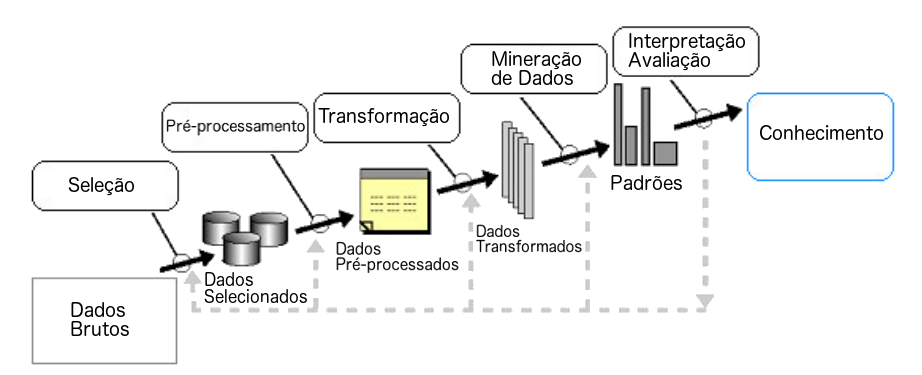
\includegraphics[width=1\textwidth]{figuras/kdd2.png}
		\caption{Passos do processo KDD, adaptado de \citeonline{fay1996}.}
		\label{kdd}
	}
	\end{figure}
	A etapa da Mineração de Dados é o mapeamento dos dados referentes a alguma informação, a validade das mesmas está atrelada ao domínio da aplicação e dos objetivos do usuário, segundo \citeonline{fay1996}. Pode ser utilizada para prever novas entradas de dados baseado nos dados já existentes e extrair informações por critérios pré-estabelecidos informando o tipo da informação ou de dado, dentre outros modelos como os estatísticos e de aprendizagem de máquina. Conforme \citeonline{chen1996} são apresentadas categorias de Mineração de Dados baseadas no tipo de informação tomada dos dados: 

	\begin{itemize}
	\item \textbf{Regras de Associação:} Encontra a frequência em que a presença de um item, em um registro, implica na presença de outros itens no mesmo registro, indicando combinações ou associações. A procura utiliza os parâmetros, onde uma regra de associação ``se existe X então existe Y'' tem uma confiança `c' e um suporte `s' no qual, a porcentagem de `c' significando o quanto ocorre esta relação e a porcentagem de `s' o quanto X ou Y aparecem nos dados.
	\item \textbf{Classificação de dados:} Os dados são separados em classes, definidas pelos conteúdos de alguns atributos, criadas de um subconjunto de treinamento.
	\item \textbf{Agrupamento (Clustering) de Dados:} Os dados são agrupados, sem uma pré-separação em classes, sendo assim, denominada classificação não supervisionada. Os agrupamentos são feitos dando preferência à similaridades de atributos dentro da classe do que entre as classes, identificando, de acordo com medidas de distância, regiões mais povoadas que são denominadas clusters.
	\item \textbf{Pesquisa por similaridade baseada em padrões:} Pesquisa por atributos similares espaciais e temporais identificando risco, causalidade e tendências associadas ao padrão. Estas informações são importantes para diversas áreas financeiras, meteorológicas e médicas. Tais atributos não precisam ser exatamente idênticos mas ter algum nível de similaridade.
	\end{itemize}
	
	Além da necessidade de extrair informações relevantes de bases de dados, é importante que exista um meio para apresentá-las, para isso são atreladas técnicas de Visualização de Dados, as quais exibem os dados, buscando adiquirir mais entendimento e introspecção sobre eles, através de representações visuais como imagens \cite{rhyne2003}. Segundo \citeonline{wong1999}, com o uso das técnicas conjuntas surge o termo Mineração Visual de Dados (VDM, \textit{Visual Data Mining}), técnicas que buscam unir o refinamento da Mineração de Dados a Técnicas de Visualização com o objetivo de extrair um número ainda maior de informações, aumentando a descoberta de conhecimento, adicionando a capacidade de cognição humana a este processo.
	
	Existem inúmeras técnicas de visualização e interação, este artigo aborda algumas delas: As visualizações de Variação Temporal Uni-escala e Multi-escala \cite{shimabukuro}; \textit{Horizon Graphs} \cite{horizon}; Foco+Contexto \cite{do2005visualizacao}; \textit{Linking and Brushing} \cite{kosara2003interaction}.
	
	\subsection{Variação Temporal Uni-escala}
		\hspace{13pt}
	\citeonline{shimabukuro} propõe um modelo que pode se aplicar para atributos que apresentam uma variação temporal em uma escala definida(dia, semana, ano, etc) utilizando uma tabela de cores, para mapear os intervalos de valores em interesse nas mesmas. Tais valores podem ser representados por sequências de pixels ou pontos, organizados em células, como na Figura~\ref{fig_uni}. O autor descreve que cada sequência de pixels é correspondente a um objeto espacial, arranjados verticalmente ou horizontalmente. Esta técnica permite uma visão simultânea de vários objetos referentes ao seu valor durante o intervalo de tempo.
	
	\begin{figure}[!h]
		{\centering
			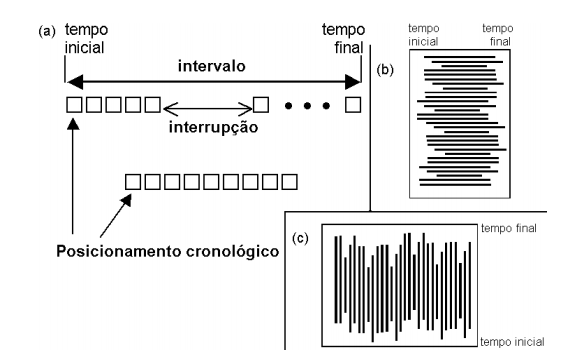
\includegraphics[width=1\textwidth]{figuras/uni.png}
			\caption{Construção da representação visual Variação Temporal Uni-escala, (a) exibe o posicionamento das células de forma cronológica presentes dentro de cada faixa que representa os dados de um objeto, (b) exibe a visualização das faixas de objetos com orientação horizontal, (c) exibe a visualização das faixas de objetos com orientação vertical,  fonte: \cite{shimabukuro}.}
			\label{fig_uni}
		}
	\end{figure}
	
	\subsection{Variação Temporal Multi-escala}
		\hspace{13pt}
	A técnica multi-escala é similar a uni-escala, porém ao invés de ter o foco em observar vários objetos ao longo do tempo, ela tem o foco em observar apenas um objeto, com um detalhamento temporal mais específico. Neste caso, são agrupados os valores do objeto em diferentes escalas de tempo na mesma visualização, permite observar os valores diários, mensais, anuais e no decorrer dos anos de tal objeto como na Figura~\ref{fig_multi}, cada coluna da visualização representa um ano, as primeiras doze células dessa coluna contém de vinte e oito à trinta e uma sub-células cada, contendo o valor diário dos dados, as próximas doze células da coluna contém o valor mensal dos dados e a última célula contém o valor anual dos dados \cite{shimabukuro}. 
	
	\begin{figure}[!h]
		{\centering
			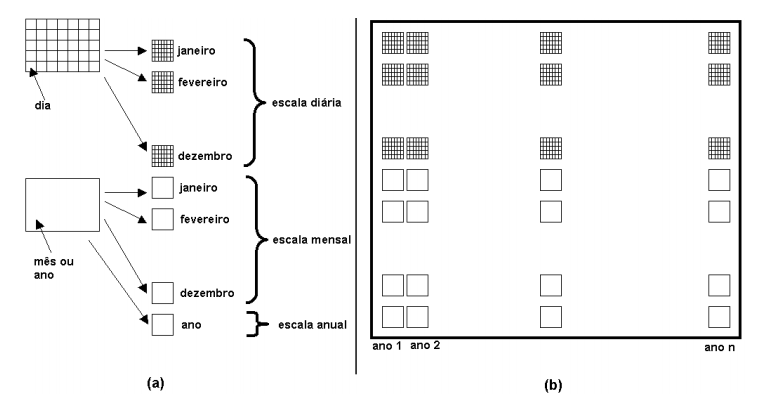
\includegraphics[width=1\textwidth]{figuras/multi.png}
			\caption{Construção da representação visual `Variação Temporal Multi-escala', (a) exibe o conteúdo detalhado dentro de cada escala, (b) exibe a visualização com todas as escalas arranjadas juntas, fonte: \cite{shimabukuro}.}
			\label{fig_multi}
		}
	\end{figure}

	\subsection{\textit{Horizon Graphs}}
		\hspace{13pt} 
	Segundo \citeonline{perin2013interactive} está é uma técnica de visualização que foi primeiro desenvolvida pelo nome de \textit{two-tone pseudo-coloring} \cite{saito2005two} e, posteriormente, foi redesenhada e renomeada pela empresa Panopticon. De acordo com \citeonline{perin2013interactive}, na construção desta visualização, primeiro os valores de cada dado são plotados em um eixo x,y. O gráfico formado é dividido horizontalmente por um valor base passado como parâmetro, valores acima deste vão ser considerados positivos e coloridos de uma cor, e valores abaixo serão considerados negativos e coloridos com outra cor, como na Figura~\ref{horizon_graph} (a). Então divide-se novamente horizontalmente por um número de faixas também passado como parâmetro. Para cada faixa é adicionada uma intensidade na cor presente iterativamente, como na Figura~\ref{horizon_graph} (b). Os valores negativos são espelhados, como na Figura~\ref{horizon_graph} (c). Por fim as faixas são recolocadas na linha do valor base, como na Figura~\ref{horizon_graph} (d). Este tipo de visualização permite representar vários gráficos em um espaço reduzido. Esta construção é exibida na Figura~\ref{horizon_graph}.
	
	\begin{figure}[h!]
	{\centering
		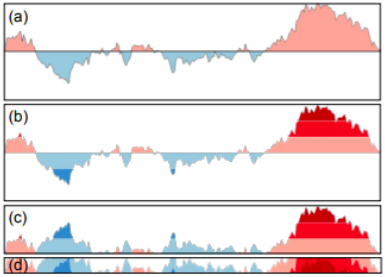
\includegraphics[width=\linewidth/2]{figuras/horizon_graph.png}
		\caption{ Construção do Horizon Graph, (a) plot dos dados no eixo x,y e divisão dos valores por valor base com colaração diferente para valores acima e abaixo do valor base, (b) divisão dos valores em faixas com intensidades de cor diferentes, (c) espelhamento dos valores negativos para cima do valor base, (d) reposicionamento das faixas divididas à partir da linha do valor base, fonte: \cite{perin2013interactive}.}
		\label{horizon_graph}
	}
	\end{figure}	
	
	\subsection{Foco+Contexto}
		\hspace{13pt}
	Segundo \citeonline{do2005visualizacao}, \citeonline{lamping1995focus} e \citeonline{card1999readings}, técnicas deste tipo permitem uma visualização geral dos dados bem como destaque em um grupo dos dados. Permitindo um foco em um conjunto específico de dados sem perder informações dos mesmos no contexto geral. Algumas aplicações dessa técnica são: Perspective Wall, ilustrada na Figura~\ref{pers_wall}, que mostra um calendário onde é possível navegar entre os meses mostrando os três meses consecutivos em foco \cite{mackinlay1991perspective}; Fish-Eye, ilustrada na Figura~\ref{fish_eye} que exibe os dados com uma escala aplicada na região de interesse \cite{bederson2000fisheye} e Table Lens, ilustrada na Figura~\ref{table_lens}, que exibe uma tabela com múltiplo foco em diferentes regiões com sorteio de múltiplas colunas a serem reveladas \cite{rao1994table} .
	
	
	\begin{figure}[!h]
	{\centering
			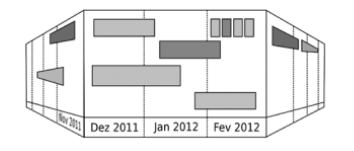
\includegraphics[width=\linewidth/2]{figuras/pers_wall.png}
			\caption{Perspective Wall aplicado a um calendário, exibe os três meses em foco à frente, nas laterais exibe os meses anteriores e posteriores aos três meses, fonte: \cite{mackinlay1991perspective}.}
			\label{pers_wall}
	}
	\end{figure}	


	\begin{figure}[!h]
	{\centering
		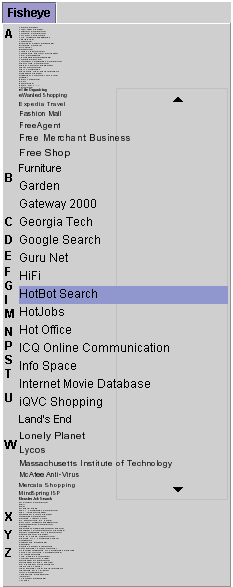
\includegraphics[height=0.5\linewidth]{figuras/fish_eye.png}
		\caption{Fisheye aplicado a uma lista de nomes, os nomes em foco estão com uma escala de aumento gradual do ponto de menor foco ao ponto de maior foco, fonte: \cite{bederson2000fisheye}.}
		\label{fish_eye}
	}
	\end{figure}



	\begin{figure}[!h]
	{\centering
		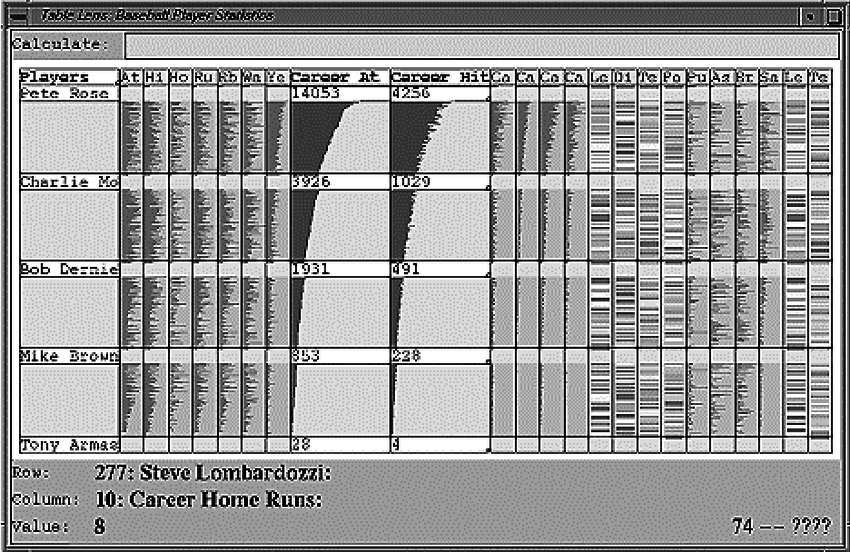
\includegraphics[width=0.7\textwidth]{figuras/table_lens2.png}
		\caption{Table Lens exibindo três colunas de quatro registros, fonte: \cite{pirolli}.}
		\label{table_lens}
	}
	\end{figure}	

	\newpage
	\subsection{\textit{Linking and Brushing}}
		\hspace{13pt}
	Esta é uma técnica de coordenação segundo \citeonline{kosara2003interaction},  \textit{Brushing} é a capacidade de selecionar valores e regiões de interesse, para serem observados na visualização. \textit{Linking} é a conexão das informações que estão sendo visualizadas em todas as visualizações, quando múltiplas delas estão sendo apresentadas. O uso dessas duas técnicas combinadas permite a seleção de quais conjuntos serão visualizados e todas as visualizações conectadas apresentarão esta informação selecionada no seu próprio modelo. Por serem usalmente implementadas juntas, tornou-se um termo só \textit{Linking and Brushing}. Pode-se ver um exemplo na Figura~\ref{link_brush} com múltiplas janelas exibindo dados médicos, compartilhando a mesma cor para os diagnósticos selecionados para a observação no gráfico, na tabela e no histograma.

	\begin{figure}[!htb]
		{\centering
			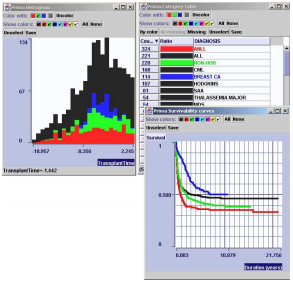
\includegraphics[width=\linewidth/2]{figuras/link_brush.png}
			\caption{\textit{Linking and Brushing} aplicado a dados médicos, exibindo um histograma, um gráfico e uma tabela que representam o mesmo conjunto de dados selecionados, fonte: \cite{kosara2003interaction}.}
			\label{link_brush}
		}
	\end{figure}	

	\section{Banco de Dados Não Relacionais - NoSQL}	
	\hspace{13pt}
	Conforme \citeonline{strauch}, os bancos de dados relacionais são os tipos predominantes para o armazenamento de dados estruturados, desde 1970. Este tipo de base de dados se suporta em uma aritmética relacional com o proliferado uso do SQL(\textit{Structured Query Language}) para inserir, alterar, recuperar e remover os dados. Bases de dados não relacionais eram utilizadas apenas para aplicações de algum nicho específico como projetos utilizando SOAP\footnote{https://www.w3.org/TR/soap/, acessado em 7 de Agosto de 2017}(\textit{Simple Object Access Protocol}) que utiliza o padrão XML\footnote{https://www.w3.org/TR/REC-xml/, acessado em 7 de Agosto de 2017}(\textit{Extensible Markup Language}), porém o uso exclusivo do SQL tem sido questionado tanto pelas empresas como pelos acadêmicos devido ao aumento de usuários e volume de dados no meio. Seguindo a argumentação dos autores, para suprir essa demanda algumas alternativas começam a ser propostas, vários outros modelos são criados para abranger mais nichos antes dominados pelos SGBDRs(Sistema Gerenciador de Banco de Dados Relacionais), esses modeloss adotam caminhos não relacionais nem sempre garantindo a ACID (Atomicidade, Consistência, Isolamento e Durabilidade) dos dados, porém conseguem otimizar o espaço de armazenamento e a performance das bases de dados, não necessariamente se desfazendo do uso do SQL.
	
	Existem dois pontos de vista não equivalentes sobre o princípio do NoSQL, uma visão apresenta o termo \textit{NoSQL} sendo \textit{No SQL} (Não SQL) que significaria uma base de dados sem SQL \cite{nosql}. Conforme \citeonline{weber} tem-se outro ponto de vista sendo \textit{NoSQL} como \textit{Not only SQL} (Não apenas SQL), ou seja, base de dados que não seja baseada em SQL porém, pode incluir ou não funcionalidades SQL, podendo existir uma abordagem híbrida. Dentro destes conceitos existem diferentes tipos de orientação para o armazenamento: Orientado a Colunas, orientado a Grafos, orientado a Documento e armazenamento baseado em Chave-Valor. Na Seção~\ref{orient_doc} será aprofundado o tipo orientado a Documento, pois foi o tipo utilizado neste projeto.
	
	\subsection{Armazenamento orientado a Documento}
		\label{orient_doc}
		\hspace{13pt}
	Segundo \citeonline{weber}, este tipo de armazenamento deve ler e escrever em algum tipo conhecido de arquivo e(ou) estrutura. Utiliza documentos com diferentes tipos de conjuntos de dados, alguns tipos de documento são de fácil interpretação para humanos, dentre eles: XML e JSON. O tipo JSON será melhor abordado na Seção~\ref{postgresql_sub_sec}. Também é possível acessar e alterar diretamente tais documentos pelo servidor.
	
	Não existe um esquema pré-definido, o que existe nas bases é a estrutura utilizada no próprio conteúdo do arquivo, sem relação nenhuma dentre os documentos da base, cada documento funciona independente do outro, no caso de bases que os arquivos dependem são chamadas de semi-estruturadas.
	
	Como a estrutura dos arquivos é algo arbitrário, campos sem dados não precisam ser preenchidos, e nenhum espaço de armazenamento precisa ser reservado. Dentre as ferramentas que o implementam estão: CouchDB\footnote{http://couchdb.apache.org/, acessado em 13 de Abril de 2016} e MongoDB5\footnote{https://www.mongodb.com/, acessado em 13 de Abril de 2016}. Exemplo de um arquivo em CouchDB  na Figura~\ref{couch}, nele está contido um elemento que contém as chaves ``\underline{ }id'' e ``\underline{ }rev'', de valores textuais, a chave ``\textit{yet\underline{ }another\underline{ }atribute}'', de valor numérico, e a chave ``\textit{\underline{ }attachements}'', que contém um subelemento como valor, as chaves deste subelemento contém outros subelementos como valor, sendo eles os dados sobre um arquivo de imagem e os dados sobre um arquivo binário.
	
	\begin{figure}[!htb]
		\centering
		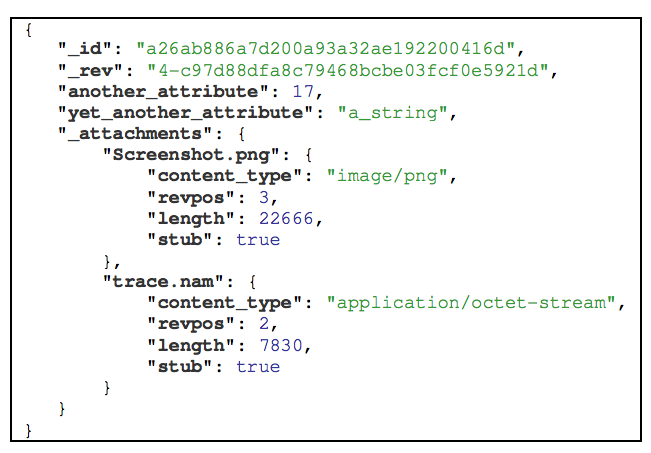
\includegraphics[width=0.7\textwidth]{figuras/doc}
		\caption{Exemplo de um documento JSON em CouchDB, fonte: \cite{weber}.}
		\label{couch}
	\end{figure}
	
	\subsection{PostgreSQL e os tipos de dados não relacionais} \label{postgresql_sub_sec}
		\hspace{13pt}
	PostgreSQL é um sistema gerenciador de banco de dados relacional bem estabelecido, com mais de 15 anos de desenvolvimento. Garante ACID e suporta a maioria dos tipos de dados SQL:2008. Tendo também o conjunto de funcionalidades dos SGBDs mais modernos como: triggers, chaves estrangeiras, views e joins. Também tem adotado algumas funcionalidades NoSQL buscando fornecer mais alternativas reunidas em uma base só, evitando que um serviço tenha que usar uma base SQL para parte de sua funcionalidade e outra base NoSQL para outro grupo de funcionalidades, permitindo uma abordagem híbrida, com suporte aos formatos JSON e XML \cite{postgresql}.
	
	Os tipos JSON e JSONB, que são orientados a Documento baseado na notação JavaScript, são utilizados como forma de armazenamento e troca de dados entre várias plataformas WEB e dispositivos móveis.
	
	JSON \textit{JavaScript Object Notation}, é um formato de dados de fácil leitura e escrita para os humanos, e de fácil geração e análise para as máquinas. Um objeto em JSON é um conjunto de pares do tipo chave-valor que podem ser organizados de forma aninhada, ou seja de forma hierárquica, e(ou) listados em arrays, a chave é uma string e o valor pode ser uma string, um número, um booleano, um array e até mesmo outro objeto aninhado. O array pode ter valores dos mesmos tipos citados. Pode haver também uma lista de objetos no mesmo nível, esta lista pode obedecer ou não a sua ordem \cite{json}.
	
	O termo JSONB é a junção de JSON com \textit{Binary}, é a serialização de documentos JSON para binário. Foi desenvolvido para melhorar o desempenho na busca das chaves utilizando sua própria ordenação indexada. Uma grande diferença para o JSON é o uso de tipos de dados com definição de tamanho e tipo pré-determinadas. Para armazenar um número inteiro o JSON utiliza uma cadeia de caracteres arbitrária enquanto o JSONB utiliza 32 ou 64 bits para inteiros e 64 bits para double e floats. O Tipo booleano em JSON é representado pela cadeia de caracteres``True'' ou ``False'', em JSONB é representado por apenas um bit 0 ou 1. Para valores como cadeias de strings são armazenadas meta- informações como o comprimento dela e, como os outros tipos já tem comprimentos definidos, um parsing na busca por uma chave pode facilmente saltar para posições do conteúdo da mesma dentro do documento \cite{postgresql}.
	
	Para utilizar os atributos JSON e JSONB foram desenvolvidos novos operadores que podem ser vistos na Tabela~\ref{json_tb} e funções auxiliares que podem ser observados na Tabela~\ref{func_tb}.
	
	\begin{table}[h!]
		\centering
		\caption{Operadores de JSON e JSONB, adaptado de \cite{postgresql}}
		\label{json_tb}
		\begin{adjustbox}{max width=\textwidth}
		\begin{tabular}{|c|c|p{5cm}|c|c|}
			\hline
			Operador & Operando à Direita & Descrição & Exemplo & Resultado do Exemplo 
			\\ \hline
			-\textgreater & int & Retorna o elemento do \textit{array} JSON & `[``a'', ``b'', ``c'']'::json-\textgreater2 & c
			\\ \hline
			-\textgreater & text & Retorna o objeto da chave & `\{``a'': [1, 2, 3]\}'::json-\textgreater`a' & [1, 2, 3]
			\\ \hline
			-\textgreater\textgreater & int & Retorna o elemento do \textit{array} JSON como texto & [`a', `b', `c']::json-\textgreater\textgreater1 & `b'
			\\ \hline
			-\textgreater\textgreater & text & Retorna o objeto da chave como texto & `\{``a'': [1, 2, 3]\}'::json-\textgreater\textgreater`a' & `[1, 2, 3]'
			\\ \hline
			\#\textgreater & text[] & Retorna o objeto JSON no caminho & `\{``a'':\{``b'': 2\}\}'::json\#\textgreater`\{a,b\}' & 2
			\\ \hline
			\#\textgreater\textgreater & text[] & Retorna o objeto JSON como texto no caminho & `\{``a'':\{``b'': 2\}\}'::json\#\textgreater\textgreater`\{a,b\}' & 2
			\\ \hline
			
		\end{tabular}
		\end{adjustbox}
	\end{table}

	\begin{table}[!h]
		\centering
		\caption{Algumas funções para processar JSON, adaptado de \cite{postgresql}}
		\label{func_tb}
		\begin{adjustbox}{max width=\textwidth}
			\begin{tabular}{|p{5cm}|c|p{5cm}|c|c|}
				\hline
				Função & Tipo de Retorno & Descrição & Exemplo & Resultado do Exemplo 
				\\ \hline
				json\underline{ }array\underline{ }length(json)
				jsonb\underline{ }array\underline{ }length(jsonb) & int & Retorna número de elementos do \textit{array} JSON & json\underline{ }array\underline{ }length(`[1, 2, 3, 4, 5]') & 5
				\\ \hline
				json\underline{ }object\underline{ }keys(json)
				jsonb\underline{ }object\underline{ }keys(jsonb) & Conjunto de texto & Retorna o conjunto de chaves do objeto JSON &json\underline{ }object\underline{ }keys(`\{``a'': 1, ``b'': 2, ``c'': 3\}') & (`a';`b';`c')
				\\ \hline
				json\underline{ }array\underline{ }elements(json)
				jsonb\underline{ }array\underline{ }elements(jsonb) & Conjunto de JSON & Retorna o conjunto de valores do \textit{array} JSON &json\underline{ }array\underline{ }elements(`[\{``a'': 1\}, \{``b'': 2\}, \{``c'': 3\}]') & (\{``a'': 1\}; \{``b'': 2\}; \{``c'': 3\})
				\\ \hline
				
			\end{tabular}
		\end{adjustbox}
	\end{table}
	\newpage
	Os tipos JSON e JSONB podem ser criados como um atributo qualquer de qualquer tabela, basta identificar o tipo após o nome do campo, como pode ser visto no Código~\ref{cria_tabela}.

	\begin{lstlisting}[
		label=cria_tabela,
		caption={Criação de uma tabela utilizando atributos JSON e JSONB},
		frame=single
	]
CREATE TABLE eventos ( 
	attrJSON JSON,
	attrJSONB JSONB,
	...
); 
	\end{lstlisting}
	
	A inserção também ocorre como em outros atributos de uma tabela, a diferença nesse caso é o conteúdo da coluna, como pode ser visto no Código~\ref{insere_tabela}.
	
	\begin{lstlisting}[
		label=insere_tabela,
		caption={Inserção em uma tabela utilizando atributos JSON e JSONB},
		frame=single
	]
INSERT INTO eventos values(
	`{``nome'': ``festa''}'::JSON,
	`{``listaDeConvidados'': 
		[``Joao'', ``Maria'', ``Roberto'']
	}'::JSONB,
	...
);
	\end{lstlisting}
	
	Pode-se utilizar os operadores e funções dentro do \textit{SELECT} e cláusulas \textit{WHERE}. A consulta abaixo recupera todas as tuplas de eventos com as colunas id e a lista de convidados onde o nome do evento seja festa, como pode ser visto no Código~\ref{consulta_tabela}.
	
	\begin{lstlisting}[
	label=consulta_tabela,
	caption={Consulta em uma tabela utilizando atributos JSON e JSONB},
	frame=single
	]
SELECT id, attrJSONB->`listaDeConvidados' 
FROM eventos 
WHERE attrJSON->>`nome' = `festa'
	\end{lstlisting}
	
	\section{Abordagem realizada}
		\hspace{13pt}
	A abordagem realizada consistiu na construção de uma aplicação WEB, portanto que pudesse ser acessada por navegadores, para uma visualização interativa de dados pluviométricos já obtidos de estações de medição presentes no estado de São Paulo. 
	Conforme mostra a Figura~\ref{ambiente}, pode-se observar o uso de diferentes tecnologias para a construção deste ambiente, e que a interação entre a aplicação WEB e os navegadores segue o esquema cliente-servidor, ou seja, os navegadores, que são os clientes, realizam as requisições e o servidor da aplicação WEB envia as respostas. Para armazenar os dados foi utilizado o SGBD PostgreSQL, com o auxílio de atributos NoSQL utilizando JSONB. O serviço WEB foi feito na linguagem Python com o \textit{framework} Django\footnote{https://www.djangoproject.com/, acessado em 7 de Agosto de 2017}, isto permitiu um encapsulamento para lidar com requisições HTTP(\textit{Hyper Text Transfer Protocol}) e ao lidar com a comunicação no Banco de Dados. O serviço WEB recebe requisições de navegadores e retorna páginas WEB como resposta, ou apenas dados no formato JSON dependendo da requisição. Esta configuração está no lado do servidor.
	No lado do cliente, os navegadores fazem as requisições ao servidor, e interpretam as páginas WEB que são encaminhadas como resposta. As páginas WEB são construídas com HTML\footnote{https://www.w3.org/html/, acessado em 9 de Agosto de 2017}(\textit{HyperText Markup Language}), CSS\footnote{https://www.w3.org/TR/REC-CSS2/cover.html, acessado em 7 de Agosto de 2017}(\textit{Cascading Style Sheets}) e JavaScript que são interpretados pelo navegador. Foi utilizada a biblioteca JavaScript D3.js para gerar as visualizações em imagens SVG. A biblioteca utiliza toda a estrutura e o estilo da página para construir as imagens.

	\begin{figure}[!h]
		\centering
		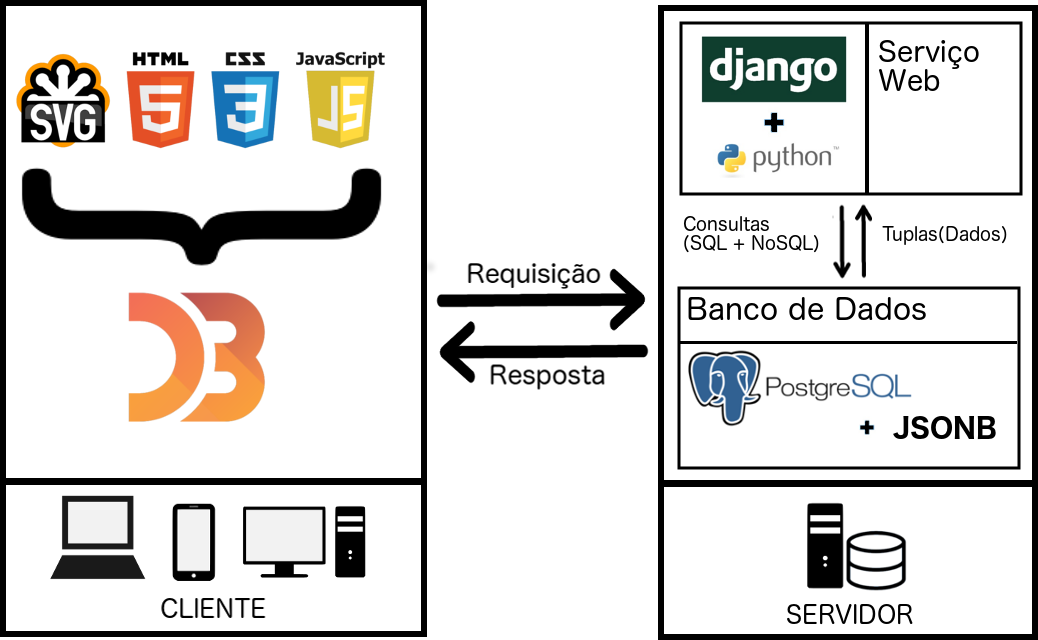
\includegraphics[width=1\textwidth]{figuras/ambiente3}
		\caption{Estrutura do projeto.}
		\label{ambiente}
	\end{figure}
	
	Inicialmente, os dados estavam em arquivos CSV\footnote{http://creativyst.com/Doc/Articles/CSV/CSV01.htm, acessado em 7 de Agosto de 2017}(\textit{Comma-separated values}), os arquivos escolhidos estavam em dois padrões, um para os dados sobre chuvas e o outro para os dados sobre as estações de medição.
	
	Os dados sobre chuvas estavam em arquivos onde o nome do arquivo é o prefixo da estação que foi feita a coleta, o prefixo, além de identificar a estação, identifica a seção e subseção da estação, ele pode ser expresso pela expressão regular: \^{}[A-Z][0-9]-[0-9][0-9][0-9]\$. A letra representa a seção e o primeiro dígito que a acompanha seria a subseção. A primeira linha do arquivo indica o número de colunas das próximas linhas, a segunda linha identifica o valor de cada coluna, as seguintes linhas contém os dados separados por colunas ano, mês e quantidade de chuva dos dias, sendo cada linha um mês de um ano, a quantidade 9999 de chuvas representa a inexistência da coleta de dados na data, esta estrutura pode ser observada na Figura~\ref{csv1}.
	
	\begin{figure}[!h]
		\centering
		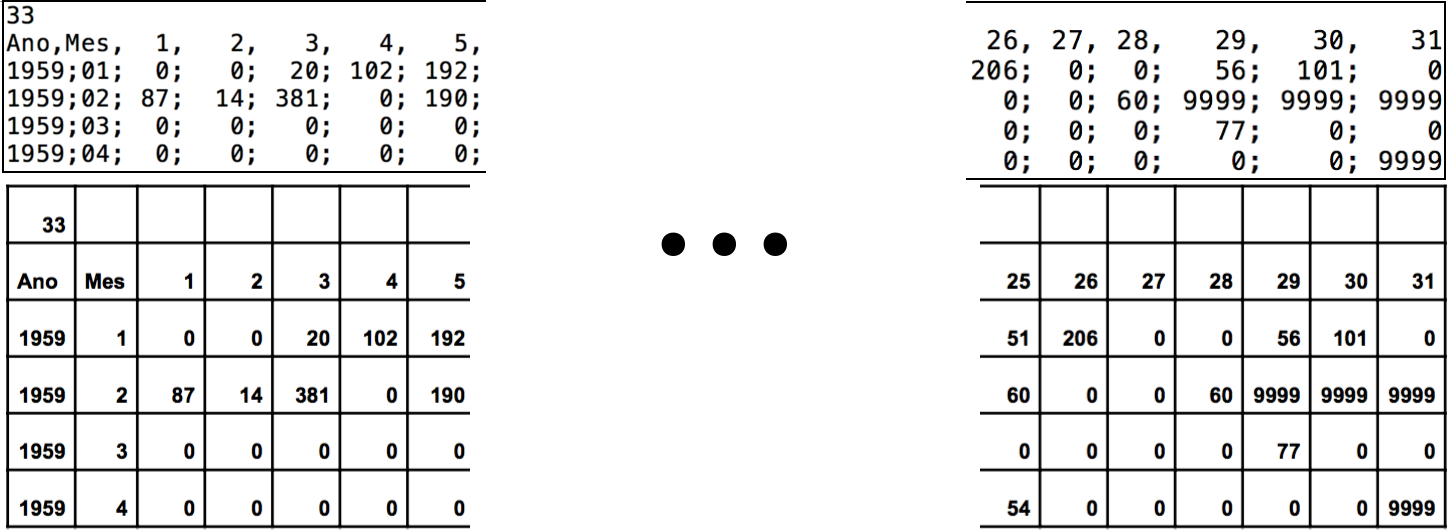
\includegraphics[width=1\textwidth]{figuras/csv1_done3}
		\caption{Parte de um arquivo CSV com dados de chuvas em texto plano e formatado em tabela.}
		\label{csv1}
	\end{figure}

	O arquivo escolhido para obter informações sobre as estações têm como primeira linha o número de colunas das próximas linhas, a segunda linha identifica o valor de cada coluna, as seguintes linhas contém, separados por colunas, os dados sobre prefixo, nome, município, bacia hidrográfica, altitude, latitude, longitude, ano Inicial da coleta, ano final da coleta, tamanho do intervalo de anos e consistência, que significa se aqueles dados foram confirmados como reais, cada linha corresponde a uma estação, esta estrutura pode ser observada na Figura~\ref{csv2}.
	
	\begin{figure}[!h]
		\centering
		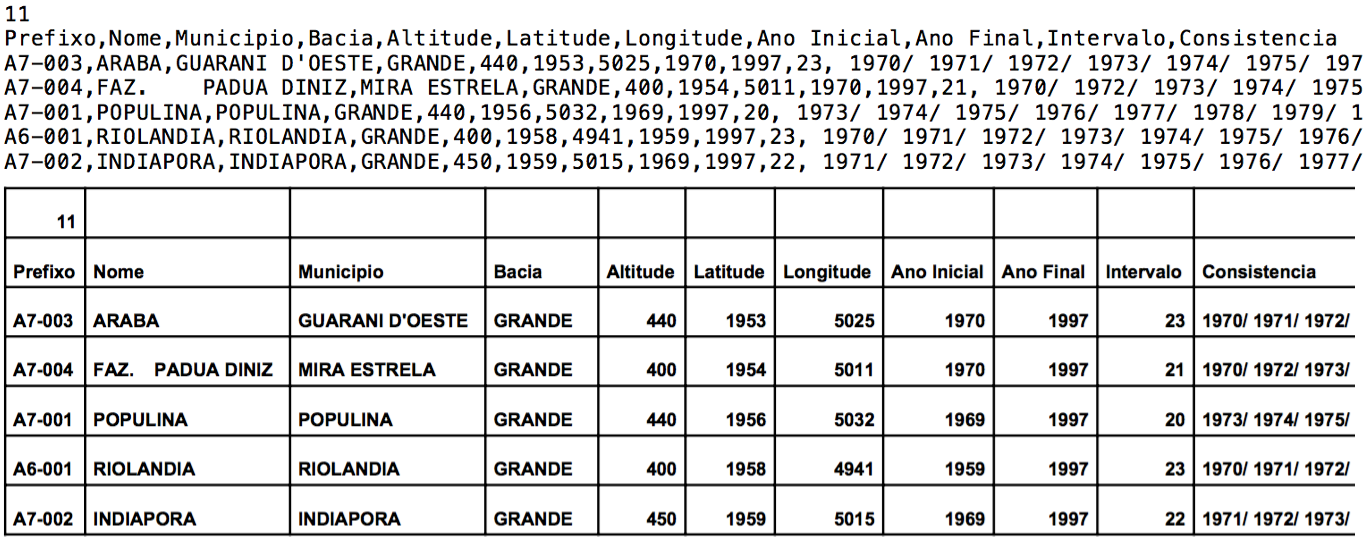
\includegraphics[width=1\textwidth]{figuras/csv2_done1}
		\caption{Parte de um arquivo CSV com dados de estações em texto plano e formatado em tabela.}
		\label{csv2}
	\end{figure}

	O conteúdo destes arquivos foi remodelado em tabelas do SGBD PostgeSQL, tem-se três tabelas, uma para Seção, outra para Subseção e uma para a Estação, a configuração das tabelas pode ser observada através do esquema ilustrado na Figura~\ref{schema}.
	
	\begin{figure}[!h]
		\centering
		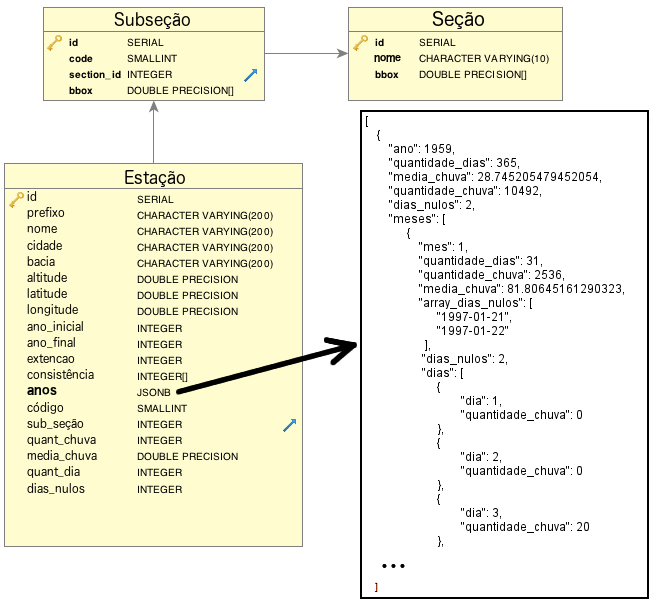
\includegraphics[width=1\textwidth]{figuras/schema3}
		\caption{Esquema construído com SQL e NoSQL(JSONB) para armazenar os dados de chuva e estações.}
		\label{schema}
	\end{figure}

	A tabela Seção contém o id e o nome da seção retirado do prefixo, a tabela Subseção contém id, nome da subseção retirado do prefixo e seção que é uma chave estrangeira para Seção, as tabelas Seção e Subseção utilizam uma coluna do tipo \textit{array} para armazenar as coordenadas do retângulo que as delimitam espacialmente, a tabela Estação contém id, subseção, que é uma chave estrangeira para a tabela Subseção, a média de chuvas da estação e todas as colunas restantes do arquivo de dados sobre a estação como atributos.

	A média de chuva mensal, anual e da estação foi calculada e adicionada aos dados no momento da inserção dos mesmos à base de dados para não ser necessário processar o cálculo destes em tempo de execução.

	Existe um atributo ``anos'' dentro da tabela Estação do tipo JSONB, ele contém os dados de chuva do arquivo de dados de chuva. Na estrutura deste atributo tem-se um \textit{array} inicial onde cada elemento corresponde a um ano, dentro do elemento ano tem-se o número do ano, a média de chuvas do ano, o número de dias daquele ano, número de dias sem dados e têm-se de forma análoga um \textit{array} de elementos meses e dentro destes um \textit{array} de elementos dias. Assim tem-se um quadro geral híbrido desta base, a recuperação destes dados é feita de diferentes formas conforme a necessidade de cada visualização, sendo este o resultado do projeto, o uso desta base para as visualizações serão abordados na Seção~\ref{testes}.

	\section{Testes e análises dos resultados}
		\label{testes}
		\hspace{13pt}
	Tem-se uma apresentação geral do resultado do ambiente na Figura~\ref{site}, foram utilizadas as visualizações Multi-escala, Uni-escala, Horizon-graph e Foco-contexto, que serão explicadas mais adiante, a visualização Foco+Contexto e o filtro de estações estão sempre visíveis, as visualizações Uni-escala, Multi-escala e Horizon-graph estão divididas em abas que podem ser alternadas.		
	
	\begin{figure}[!h]
		\centering
		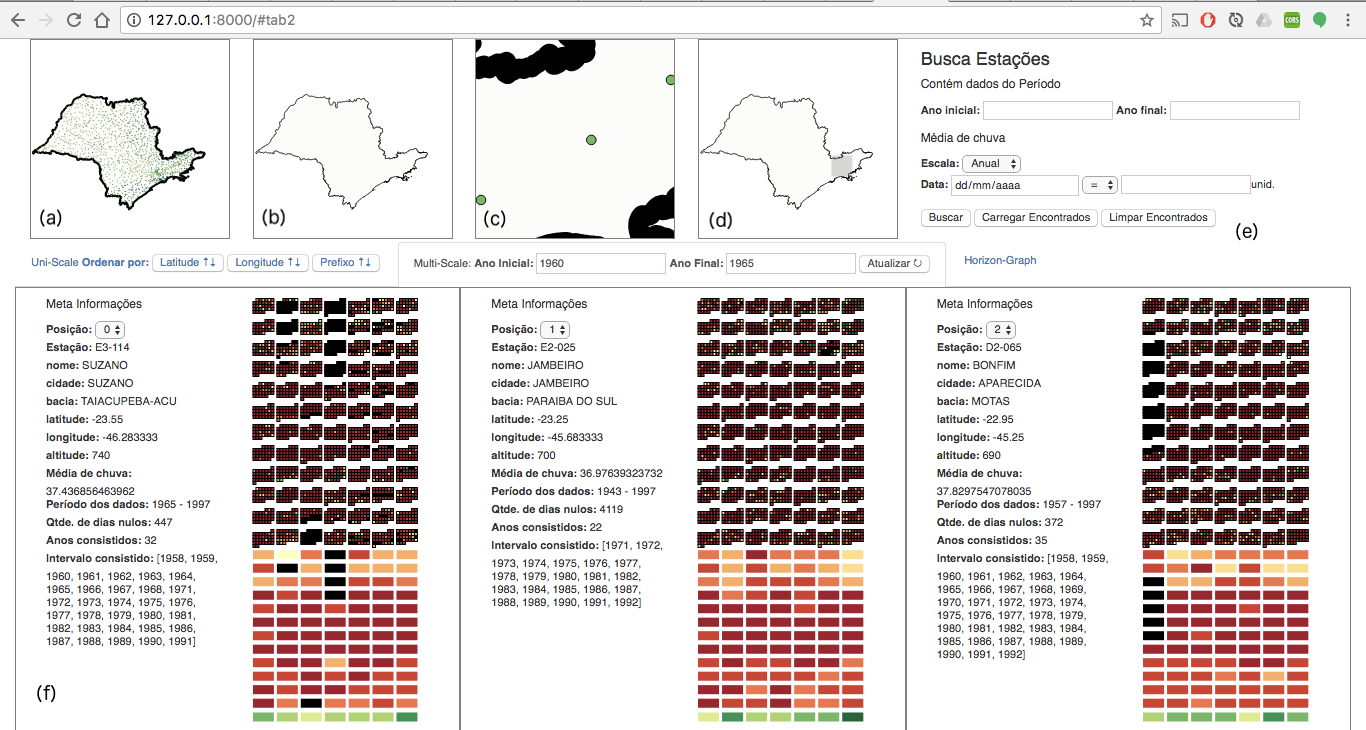
\includegraphics[width=1\textwidth]{figuras/site3}
		\caption{Aspecto geral do ambiente WEB, (a) mapa com todas as estações, (b) auxiliar para esquema Foco+Contexto de (a), (c) mapa com estações selecionadas, (d) auxiliar para esquema Foco+Contexto de (c), (e) filtro textual de estações, (f) visualizações Multi-escala das estações selecionadas.}
		\label{site}
	\end{figure}

	A biblioteca D3.js foi utilizada para construir todas as visualizações, facilitando a escrita de código, alguns laços de repetições puderam ser ignorados, pois a biblioteca utiliza os \textit{callbacks} iterativamente à quantidade de elementos dentro dos dados, realizando chamadas implícitas às funcões que executam o desenho, dados complexos em JSON puderam ser processados em todas as camadas de subelementos, e obteve-se uma flexibilidade na geração das visualizações, sendo elas adaptáveis ao conteúdo dos dados passados.
	 
	 O propósito de cada visualização e sua forma de interação serão apresentados nas próximas seções, em adicional ao conjunto de visualizações foi introduzido um filtro de estações por parâmetros textuais, o filtro utiliza uma busca híbrida com parâmetros em SQL e NoSQL na mesma consulta, este recurso também será aprofundado nas seções seguintes.
	
	Além da interatividade presente em cada visualização, foi utilizada a técnica de coordenação \textit{Linking and Brushing}, pela qual é possível, de diferentes fontes de visualizações, adicionar uma estação ao conjunto de estações selecionadas para a visualização. Pode-se adicionar a partir da visualização Uni-escala, da Foco-contexto e do filtro SQL+NoSQ, também é possível visualizar as várias estações selecionadas em várias visualizações simultaneamente.
	
	\subsection{Visualização Foco+Contexto}
		\hspace{13pt}
	No topo do ambiente à esquerda, tem-se quatro mapas do estado de São Paulo, onde espacialmente estão contidas as estações em que foram obtidas as medições pluviométricas. Os círculos representam o local das estações de medição. A cor interna dos círculos representa a média de chuvas de todos os anos da estação. Estas visualizações estão presentes para poder-se associar as informações espaciais que obtem-se delas às outras visualizações. Para esta visualização, são recuperadas todas as estações da base de dados mas com apenas os atributos que serão utilizados, eliminando principalmente o atributo anos, pois é o atributo com a maior quantidade de dados.
	
	Na Figura~\ref{site} (a), tem-se o primeiro mapa exibindo todas as estações representadas por círculos, nele são disponibilizadas algumas interações. É possível executar o efeito zoom e pan ilustrado na Figura~\ref{mapa_zoom_pan}. 
	
	\begin{figure}[!h]
		\centering
		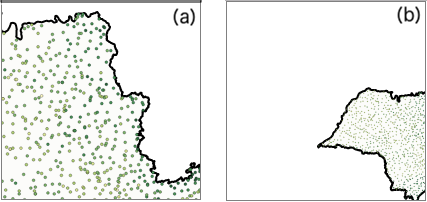
\includegraphics[width=0.4\textwidth]{figuras/mapa_zoom_pan1}
		\caption{(a) interação de zoom aplicado na Figura~\ref{site} (a), (b) interação de pan aplicado na Figura~\ref{site} (a).}
		\label{mapa_zoom_pan}
	\end{figure}
	
	O clique em um dos círculos adiciona a estação, representada pelo círculo, ao conjunto de estações selecionadas para visualização e, ara facilitar o acerto do clique, foi implementada uma escala de aumento do tamanho no círculo em que o mouse estiver sobre ele, este recurso pode ser visto na Figura~\ref{mapa_click}.
	
	\begin{figure}[!htb]
		\centering
		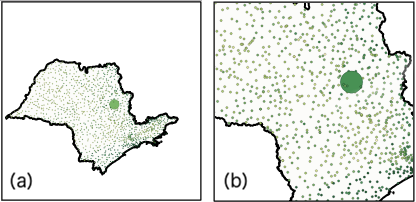
\includegraphics[width=0.4\textwidth]{figuras/mapa_click1}
		\caption{(a) aplicação de aumento de escala em estação sobre o mouse para facilitar o clique na Figura~\ref{site} (a), (b) aplicação de aumento de escala em estação sobre o mouse para facilitar o clique com interação de zoom aplicadas na Figura~\ref{site} (a)}
		\label{mapa_click}
	\end{figure}
	
	Na Figura~\ref{site} (b), tem-se o segundo mapa que é parte da visualização Foco+Contexto referente ao primeiro mapa em Figura~\ref{site} (a). É exibido o mapa completo destacando a parte visível do primeiro mapa em um retângulo com pouca opacidade. Esta visualização permite navegar no primeiro mapa através de zoom e pan sem perder a informação de onde se encontra aquela região no mapa completo. No próprio mapa da Figura~\ref{site} (b), há a interatividade de desenhar o retângulo que será a visualização do mapa da Figura~\ref{site} (a). Este comportamento pode ser observado na Figura~\ref{mapa2}.
	
	\begin{figure}[!htb]
		\centering
		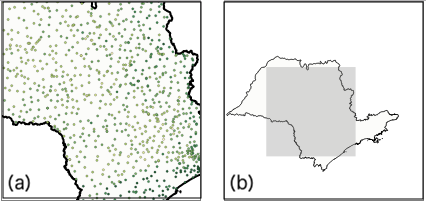
\includegraphics[width=0.4\textwidth]{figuras/mapa2_1}
		\caption{(a) interação de zoom aplicado na Figura~\ref{site} (a), (b) Figura~\ref{site} (b) exibindo a área visível no mapa completo.}
		\label{mapa2}
	\end{figure}
	
	Na Figura~\ref{site} (c), tem-se o terceiro mapa exibindo as estações que foram selecionadas. Neste mapa é calculado o retângulo menor possível que contenha as estações selecionadas, após o cálculo deste retângulo é feito o maior zoom possível na região delimitada do retângulo e, evido a este cálculo e zoom a interação de pan e zoom manual estão desabilitadas neste mapa. O quarto mapa, exibido na Figura~\ref{site} (d), segue como parte da visualização Foco+Contexto para dar apoio a visualização do terceiro mapa.
	
	\subsection{Visualização Uni-escala}
		\hspace{13pt}
	A visualização Uni-escala representa o período em que os dados estão consistidos de cada estação, o prefixo da estação a identifica, é possível adicionar a estação ao conjunto de estações selecionadas clicando no prefixo, e a lista pode ser ordenada por latitude, longitude e prefixo. O objetivo da visualização é permitir uma análise de quais estações possuem dados consistentes dentro do mesmo período para que possam ser comparadas. Os mesmos dados que foram recuperados na visualização Foco+Contexto são reaproveitados nesta, a visualização pode ser observada na Figura~\ref{uniescala02}.
	
	\begin{figure}[!h]
		\centering
		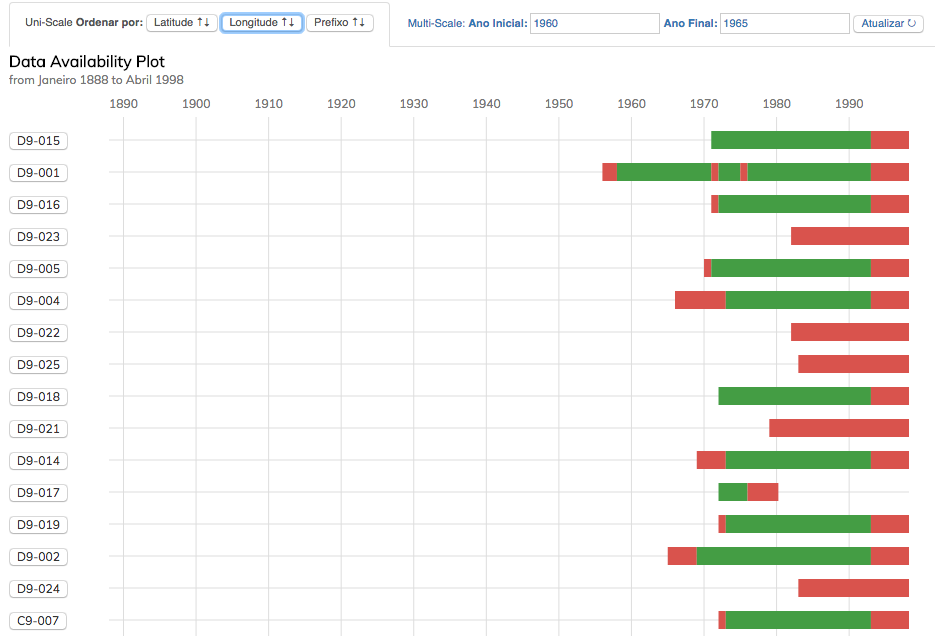
\includegraphics[width=0.99\textwidth]{figuras/uniescala02}
		\caption{Visualização Uni-escala informando a consistência dos dados dentro da escala anual.}
		\label{uniescala02}
	\end{figure}
	\newpage
	\subsection{Visualização Multi-escala}
	\hspace{13pt}
	A visualização Multi-escala exibe a quantidade de chuva durante diferentes escalas de tempo com alguns atributos textuais sobre as estações selecionadas. Nesta visualização, a cor preta significa a inexistência de dados sobre o período, e as outras cores estão dentro de uma escala entre vermelho e verde, onde cores próximas do vermelho significam valores baixos e cores próximas do verde significam valores altos. Várias estações podem ser exibidas e serão apresentadas lado a lado. Os anos que serão exibidos são editáveis na própria aba, permitindo atualizar os dados que estão sendo visualizados, como na Figura~\ref{multi_time}
	
	\begin{figure}[!htb]
	\centering
	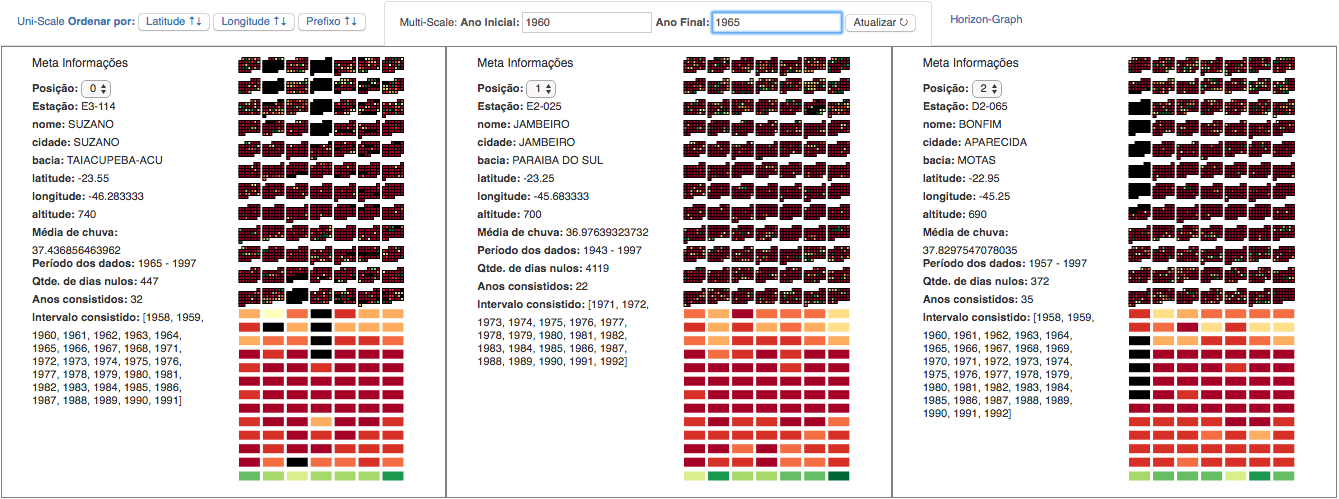
\includegraphics[width=1\textwidth]{figuras/multi_time}
	\caption{Visualização Multi-escala com seleção de intervalo de visualização.}
	\label{multi_time}
	\end{figure}

	É possível visualizar a quantidade de chuva de maneira textual ao passar o mouse por cima das células da visualização, esta interação pode ser observada na Figura~\ref{multi_tool}.
	
	\begin{figure}[!h]
		\centering
		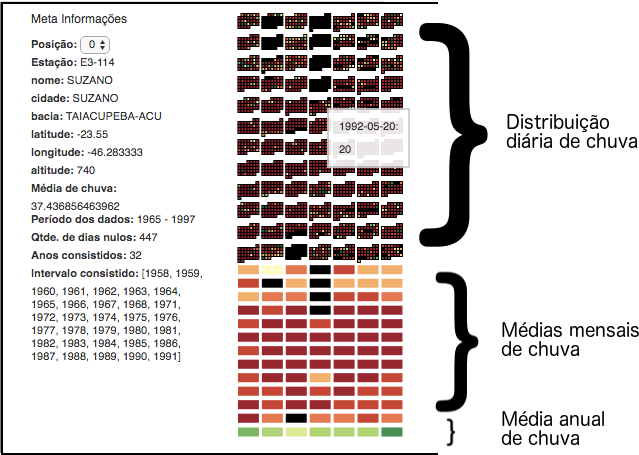
\includegraphics[width=0.8\textwidth]{figuras/multi_tool1}
		\caption{Informação textual da quantidade de chuva da célula sobre o mouse.}
		\label{multi_tool}
	\end{figure}

	Também existe a possibilidade de alterar a posição das visualizações, permitindo escolher quais estações serão visualizadas com maior proximidade visual, esta funcionalidade pode ser vista na Figura~\ref{multi_ord}.
	
	\begin{figure}[!htb]
		\centering
		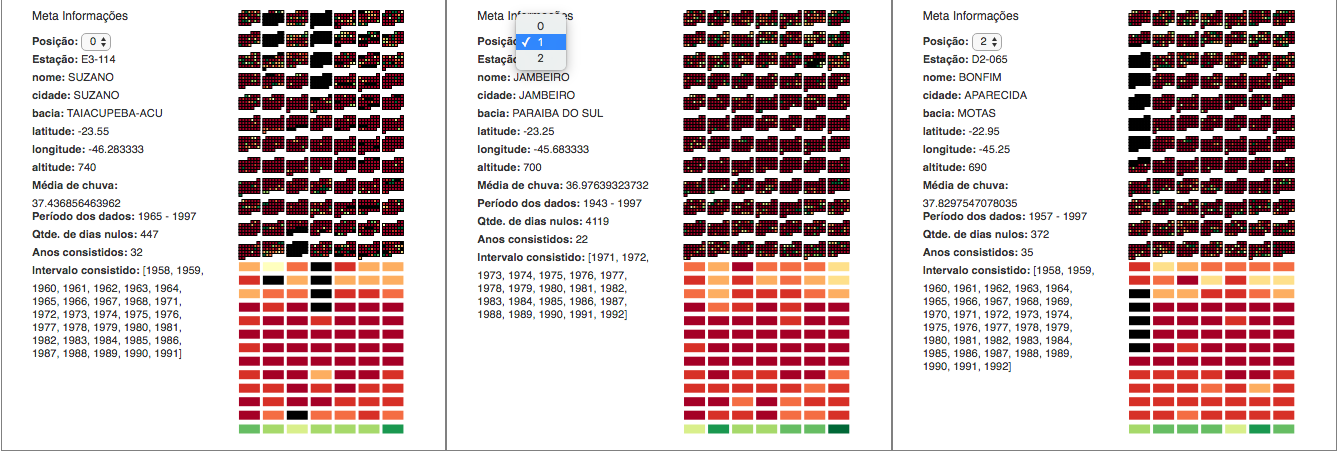
\includegraphics[width=1\textwidth]{figuras/multi_ord}
		\caption{Realocando a posição das visualizações Multi-escala.}
		\label{multi_ord}
	\end{figure}
	
	Essa visualização dá suporte para a obtenção de informações de quantidade de chuvas durante longo período de tempo sem perder micro-informações de pequenas escalas de tempo como de dias, podendo também comparar o comportamento de diferentes estações. Para gerar a visualização são recuperados todos os atributos da estação selecionada, no atributo anos ocorre uma filtragem para não carregar anos fora do intervalo a ser visualizado.
	
	\subsection{Visualização \textit{Horizon Graph}}
		\hspace{13pt}
	A visualização \textit{Horizon Graph} exibe os dados sobre a média de chuva mensal, durante o período selecionado na Multi-escala, das estações selecionadas. O foco desta visualização é exibir várias estações em um espaço verticalmente reduzido e o comportamento das chuvas ao decorrer do tempo. Os dados recuperados na visualização Multi-escala são reaproveitados nesta. No caso de dados pluviométricos não tem-se valor negativo de chuvas, e nenhum valor foi passado como valor base, logo a aplicação do \textit{Horizon Graph} não se divide em cores positivas e negativas. A visualização pode ser observada na Figura~\ref{my_horizon}.
	\begin{figure}[!htb]
		\centering
		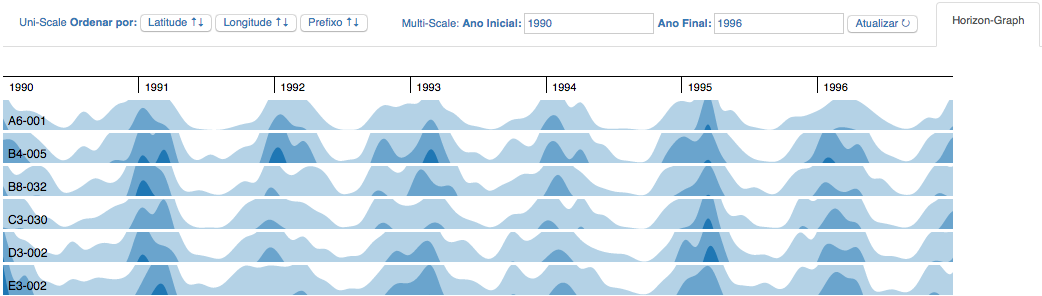
\includegraphics[width=1\textwidth]{figuras/my_horizon1}
		\caption{\textit{Horizon Graph} exibindo a média de chuva mensal durante os anos.}
		\label{my_horizon}
	\end{figure}
	
	\subsection{Filtro de estações}
		\hspace{13pt}
	No Filtro de estações é possível realizar a busca e seleção de estações, pode-se filtrar por estações em que: Contenha dados dentro do período do ano inicial ao ano final, a quantidade de chuva da escala da data seja maior, menor, maior ou igual, menor ou igual, ou igual a quantidade inserida. A busca identifica o número de estações encontradas, então é possível adicioná-las ao conjunto de estações selecionadas. O filtro pode ser observado na Figura~\ref{filtro}.
	
	\begin{figure}[!htb]
		\centering
		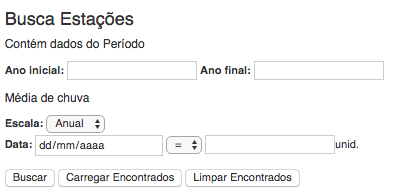
\includegraphics[width=0.5\textwidth]{figuras/filtro}
		\caption{Filtro para executar buscas textuais por estações.}
		\label{filtro}
	\end{figure}
	
	Para poder levar os resultados em todas as visualizações esse filtro carrega todos os atributos das estações filtradas. Dentre os parâmetros utilizados na filtragem tem-se os atributos SQL: data de início da coleta, data final da coleta. Estes podem ser combinados com a média de chuva presente dentro do atributo NoSQL anos. A média de chuva corresponde ao valor presente na data escolhida dentro da escala anual, mensal ou diária, exemplo: Se escolhida a data 10/07/2017 e a escala mensal, a consulta buscará a média de chuva do mês de Julho do ano de 2017 de todas as estações. Os operadores de comparação \textgreater, \textless, \textgreater=, \textless=, = são diretamente utilizados na comparação do valor da média dentro da consulta. Um exemplo da consulta híbrida pode ser observado no Código~\ref{consulta_hibrida}, esta consulta retorna as tuplas em que os dados estão consistidos entre o período de 1990 a 1996 e quando a média de chuva da data de sete de Julho de 1993 for maior do que quarenta.

		\begin{lstlisting}[
	label=consulta_hibrida,
	caption={Consulta híbrida com cláusulas WHERE verificando atributos SQL e NOSQL},
	frame=single
	]
WITH years_data AS (
	SELECT id, year_ini, year_end, st_years, prefix, code, ...
	FROM rainfall_station st, 
		jsonb_array_elements(st.years) st_years
	WHERE (st_years->>'year')::int = 1993
)
SELECT DISTINCT ON (id) id, year_ini, year_end, prefix, code, ...
	FROM years_data WHERE
	(
		st_years->'months'->6->'days'->6->>'day_average'
	)::float > 40.0
	AND year_ini <= 1990 AND year_end >= 1996
	\end{lstlisting}

	\subsection{Comparação de SQL e NoSQL}
		\hspace{13pt}
	Além de observar o resultado das visualizações, é interessante atentar para os diferenciais de uma arquitetura híbrida, podem existir diferentes formas de modelar os dados utilizados neste projeto apenas em SQL mas, para fins de comparação, foi construída somente uma modelagem apenas em SQL conforme o esquema da Figura~\ref{schema_sql}.
	
	\begin{figure}[!h]
		\centering
		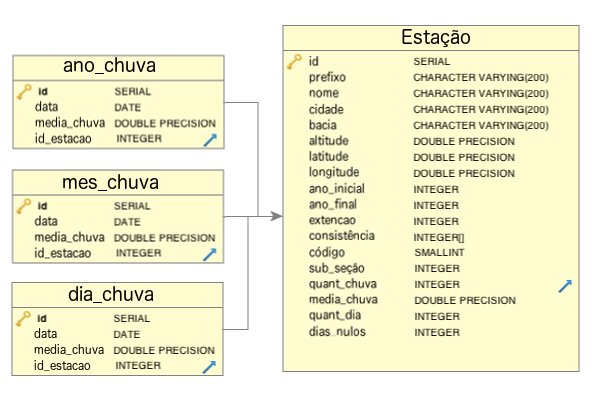
\includegraphics[width=0.78\textwidth]{figuras/schema_sql2}
		\caption{Esquema modelado em SQL para armazenar os dados de chuva.}
		\label{schema_sql}
	\end{figure}
	\newpage
	Observa-se que neste modelo apenas SQL, para encontrar o valor de chuva de um dia tem-se que primeiro pesquisar as tuplas de dia\underline{ }chuva que pertencem à estação. No modelo deste projeto, em razão do atributo JSONB anos já estar pertencente à tupla e, os dias e meses estarem indexados, tem-se um acesso direto aos dias e meses dos anos da estação. Considerando somente a quantidade de tuplas acessadas usando apenas SQL em comparação com a abordagem híbrida, com o objetivo apenas de recuperar os dados de um dia de uma estação em uma determinada data, tem-se algumas observações:
	
	\begin{itemize}

		\item No caso de apenas SQL, é necessário encontrar todas as tuplas de dia\underline{ }chuva com a chave estrangeira igual ao id da estação, como o acesso a chaves estrangeiras pode ser indexado, é possível desconsiderar este passo, então essa pesquisa percorre, no pior caso, o número de tuplas igual ao número de anos em cada estação aproximadamente, vezes 365 dias aproximadamente, avaliando que tem-se, em média, 20 anos em cada estação, o resultado seria aproximadamente 7.300 tuplas para encontrar a tupla de dia\underline{ }chuva com o atributo id da estação na determinada data.

		\item No caso do SQL com JSONB, basta verificar o id da tupla da estação desejada dentre todas as tuplas de estações, como o acesso a chaves primárias é indexado pode-se desconsiderar este passo, após encontrar a tupla, basta procurar o ano dentro do atributo anos, em média 20 elementos de um \textit{array}, acessar diretamente o mês pelo índice e, posteriormente, o dia pelo índice, desconsiderando o acesso indexado dentro do JSONB, teria apenas 20 tuplas referente ao número médio de anos mas, ainda que fossem considerados os passos indexados dentro do JSONB como se fosse o custo de acesso a tuplas na contagem, teriá-se 20 anos aproximadamente dentro da estação já encontrada vezes 2 acessos diretos indexados para mêses e dias, seria então 40 itens.
		
	\end{itemize}
	
	É importante frisar que, embora possa existir alguma outra opção de modelagem apenas em SQL para os dados utilizados no projeto, e que seja tão eficiente ou mais à modelagem híbrida, ainda pode-se analisar este tratamento de forma didática e análoga para cenários em que alguns atributos das tabelas tem valores ordenados mas que não podem ser indexados comumente em bases apenas SQL, ocasionando uma grande quantidade de tuplas para serem processadas. Além de que a pesquisa de tuplas dentro de atributos JSONB facilitou o acesso aos dados por ser possível acessá-los de chaves ou índices dentro do json ao invés de realizar \textit{subqueries}.
	
	Uma dificuldade encontrada foi o tamanho dos dados por tupla pois, todos os dados de chuva sobre a estação estão em apenas um atributo JSONB dentro da tupla, então um recurso essencial para diminuir este problema foi realizar as buscas sem selecionar o atributo JSONB. Apenas utilizá-lo dentro das cláusulas \textit{WHERE} e em casos onde é necessário a recuperação dos mesmos para as visualizações, como na visualização Multi-escala, onde ela utiliza os dados dentro do atributo JSONB, mas mesmo assim, após a recuperação dos dados, ainda é feito um corte deixando apenas os que serão utilizados na visualização.
	
	\section{Conclusões e trabalhos futuros}
		\hspace{13pt}
	Este trabalho apresentou um ambiente WEB para visualizar dados pluviométricos de forma interativa e coordenada, para isso foram utilizadas várias técnicas de visualização e várias tecnologias para dar apoio ao desenvolvimento, como o uso da biblioteca JavaScript D3.js para gerar as visualizações e aplicando uma abordagem híbrida para o armazenamento e recuperação dos dados com o PostgreSQL+NoSQL.
	
	O uso das técnicas de visualização combinadas com interação e coordenação permitiu observar diferentes informações dos dados em um mesmo contexto, e o uso de banco de dados PostgreSQL+NoSQL foi uma alternativa para solucionar os problemas de recuperação de dados dentro do grande volume utilizado neste projeto, podendo observar os benefícios e dificuldades do uso da abordagem híbrida, além da possibilidade de aplicá-la em outros contextos de aplicações de forma análoga.

	Para a continuação deste trabalho sugere-se realizar testes de usabilidade com especialistas da área de climatologia para encontrar possíveis necessidades de adaptar e(ou) adicionar visualizações, como utilizar um período para exibir a media de chuvas da estação nos mapas, e seria interessante também que fosse disponibilizado no ambiente um acesso para atualizar os dados que no momento são apenas recuperáveis.


	%\bibliographystyle{abnt}
	%\bibliographystyle{apa}
	\bibliography{referencias} 
\end{document}